\section{Introduction}
In 1928, Edward Condon introduced the useful approximation that the transition dipole moment does not depend on variations of nuclear coordinates ~\cite{Condon}. Deviations from the approximation are crucial for the explanation of Raman Spectroscopy ~\cite{ResonanceRaman}.

The Condon approximation is often employed without verifying what are the effects of lifting it. Recently, Heller and co-workers have shown that the variation in transition dipole moment is crucial to explain the Raman spectrum of graphene ~\cite{hellerGraphene}.  Furthermore, recent studies suggest a highly noticeable transition dipole moment in photosynthetic pigments ~\cite{photosyntheticKappa}.  Van Voorhis and co-workers have recently stressed the role of non-Condon effects in electron transfer ~\cite{MavrosNonCondon}.  Finally, our own work indicates that non-Condon effects may make the application of witnesses of electronic spectroscopy ~\cite{witness,allanWitness} harder than originally thought~\cite{myWitnessPaper}.

In this work, we examine the role of non-Condon effects in one of the simplest forms of spectroscopy, linear absorption spectroscopy.

\section{System Setup}
For the purposes of this work, we will employ a simple model that consists of a one-mode vibrational monomer with a ground electronic state $\ket{g}$ and an excited electronic state $\ket{e}$ and assume the vibrational frequency is the same in both states.  In principle, however, this method is extensible to more vibrational degrees of freedom.  Using this assumption, we can write the Hamiltonian for the system as,
\begin{align}
	H_0 &=  \sum_n \hbar \omega \left(n + \frac{1}{2} \right)  \ket{n_{\gamma}}\ket{g}\bra{g} \bra{n_{\gamma}} \\
   &+ \sum_m \left(  \hbar \omega  \left(m + \frac{1}{2} \right) + \omega_e \right)  \ket{m_{\epsilon}} \ket{e}\bra{e} \bra{m_{\epsilon}}
\end{align}
Here, the Greek indices corresponding to the vibrational states and the roman indices corresponding to the electronic states.  The ground and excited electronic states are represented by $\ket{g}$ and $\ket{e}$, and the set of $\ket{i_{\gamma}}$ is the set of vibrational eigenstates in the ground electronic state manifold, and $\ket{i_{\epsilon}}$ is the set of vibrational eigenstates in the electronic excited state.  The vibrational quanta is $\omega$ and $\omega_e$ is the electronic energy gap.  The electronic transition  dipole moment $\hat{\mu}$ varies spatially as a function of the x coordinate in an object $\mu(x)$,
\begin{align}
	\hat{\mu} &= \mu (x)  \left( \ket{e}\bra{g} + \ket{g} \bra{e} \right)
\end{align}
For the purposes of this study, we construct a generic polynomial transition dipole moment, which one can be expressed as ladder operators for easier calculation,
% (Al\'an, here I differed from your suggestion to just keep linear, because I realized that we do use more than just the linear moment later in the paper; let me know what you think.)
\begin{align}
	\mu(x) &= \mu_0 \sum_{i=0} \kappa_i x^i \\
	&= \mu_0 \sum_{i=0} c_i \left( \hat{a} + \hat{a}^{\dagger}\right)^i
\end{align}
or as a vibrational matrix element,
\begin{align}
	\mu_{a,b} = \bra{a_{\gamma}} \mu(x) \ket{b_{\gamma}}
\end{align}
Going forward, we will use the a notation of $(\{i\})$ to indicate the polynomial orders of $x$ we included.  In a simple linear variation setting would be,
\begin{align}
	\mu^{(1)}_{a,b} = \mu_0 \left[ \delta_{a,b} + c \left( \sqrt{b-1}\delta_{a,b-1} + \sqrt{b}\delta_{a,b+1}\right) \right]
\end{align}
but for a cubic variation would be,
\begin{align*}
	\mu^{(3)}_{0,\lambda} =& \mu_0 \left( \delta_{0,\lambda}  + c_3   \left(2\delta_{1,\lambda}  +\sqrt{6}\delta_{3,\lambda} \right)\right)
\end{align*}

Because higher-polynomial orders cascade down (meaning that $\left( \hat{a} + \hat{a}^{\dagger}\right)^3$ and )

\section{Effects on Linear Absorption Spectroscopy}
The change in transition dipole moment from the Condon approximation will not affect the frequency of the transitions in our model, so instead we look only at peak heights: specifically the absorptivity normalized to the frequency squared
\begin{align}
	\frac{\epsilon(\omega) }{\omega^2} = K(\omega) = \sum_{\eta,i} h_{\eta,i} f_{L} (\omega, \sigma, \Delta\omega_{\eta,i})
	\label{eqn:KDef}
\end{align}
where $f_{L}$ is a line-shape function which integrates to unity, sigma $\sigma$ is the width parameter(s) for the line-shape.  Finally and most importantly, $h_{\eta,i}$ and $\Delta\omega_{\eta,i}$ are the strength and frequency, respectively, of the transition from the ground vibrational state $\eta$ to the excited vibrational state $i$.


Normally a researcher can compare the $k$th and $k+1$th transition strengths to ascertain the Huang Rhys Parameter $S$:
\begin{align}
	\frac{h_{\eta,k+1}}{h_{\eta,k}} &=  \frac{\sum_{\lambda,\nu} \mu_{\eta,\lambda}^*\mu_{\eta,\nu}   O_{\lambda}^{k+1} O_{\nu}^{k+1} }{\sum_{l,n} \mu_{\eta,l}^*\mu_{\eta,n}   O_{l}^{k} O_{n}^{k} } = H(\eta,k)
	\label{eqn:HDef}
\end{align}
Where $O_{\lambda}^{k}$ is the Franck-Condon overlap factor between a electronic ground vibrational energy state $\lambda$ and an electric excited vibrational energy state $k$.  If one starts out in the 0th state and assumes constant transition dipole moment($0$th order as indicated in the subscript to $H$), the relation is quite simple:
\begin{align}
	H_{(0)}(0, k)	&= \frac{S }{k+1 }
\end{align}
But going one step further to a linear-only transition dipole variation, one obtains the relation between subsequent peak heights of
\begin{align}
	H_{(1)}(0, k)	&=  \frac{S }{k+1 } \frac{\left| 1 + c\sqrt{S} \left( 1  - \frac{k+1}{S} \right) \right|^2}{\left| 1 + c \sqrt{S} \left( 1  - \frac{k}{S} \right)\right|^2 }
\end{align}
Of crucial relevance to our argument is that if one only employs the ratio of the $0 \rightarrow 1$ peak to the $0 \rightarrow 0$ peak under the assumption of linear variation of the transition dipole moment, one is not extracting a pristine Huang-Rhys parameter, but rather an effective Huang-Rhys parameter $S_{\text{eff}}$,
\begin{align}
	S_{\text{eff}}	&=  S \frac{\left| 1 + c \sqrt{S} \left( 1  - \frac{1}{S} \right) \right|^2}{\left| 1 + c \sqrt{S} \right|^2 }
\end{align}
In Figure \ref{fig:absorpstion_HRF_error_sVerr}, we plot the potential error in the estimation of the Huang-Rhys parameter as a function of the variation of the linear dependence of the transition dipole moment.
\begin{figure}
   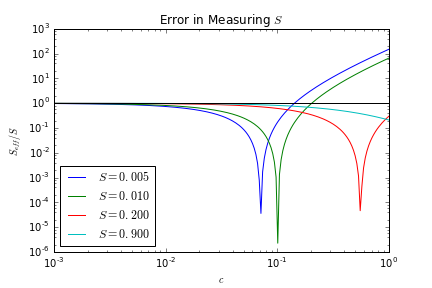
\includegraphics[width=1.0\columnwidth]{error_plot_sVerr.png}
   \caption{The relative measurement error as the ratio of the effective Huang-Rhys parameter over the actual Huang-Rhys parameter ($S_{\text{eff}} / S $ ) as a function of $S$ for the ratio of the $0\rightarrow1$ peak to the $0\rightarrow0$ peak, for various values of $S$ and an entirely real linear-variation in the transition dipole moment: $c$.  If the Huang-Rhys parameter is small, even small linear variations of the transition dipole moment with coordinate can induce large errors in its estimation.}
	\label{fig:absorpstion_HRF_error_sVerr}
\end{figure}

\section{Corrections to Tetracene}
The use of the peak heights in absorption spectra to determine the coordinate dependence of transition dipole moments has been employed for more than 60 years.  In 1954, Fraser described how to map out the precise coordinate dependence of transition dipoles in high-resolution electronic-vibrational absorption spectra of diatomics~\cite{FraserFindingNCM}.  But in solution, one often far fewer peaks so a full map is not possible.  Here we describe a method to find an approximate low-order polynomial transition dipole variation for just one mode in a molecule in solution.

To demonstrate this, we take the absorption spectrum of tetracene in dichloromethane~\cite{TetraceneDichloromethane} and in toluene~\cite{TetraceneToluene}.  We chose tetracene because of its important role in organic electronics and recently in singlet-fission studies~\cite{singletFissionVibration} and because it has a sufficiently large Huang-Rhys parameter $S$ that results in a spectrum with multiple line-shapes.

We fit Equation \ref{eqn:KDef} to the addition of 5 Voigt line-shape for the Toluene spectrum and 6 Voigt line-shapes for the DCM spectrum.  The Voigt profile allows peaks to have varying amount of Gaussian and Lorentzian line-shape character.  The results of this fit are shown in Figures \ref{fig:dcm_fit} and \ref{fig:toluene_fit}.  We then employed the centers of the line-shapes and fit a Morse oscillator model, the results of which are summarized in Table \ref{table:energyFit} which allowed us to conclude that the harmonic approximation is sufficient for an accurate description of this system.

\begin{figure}
   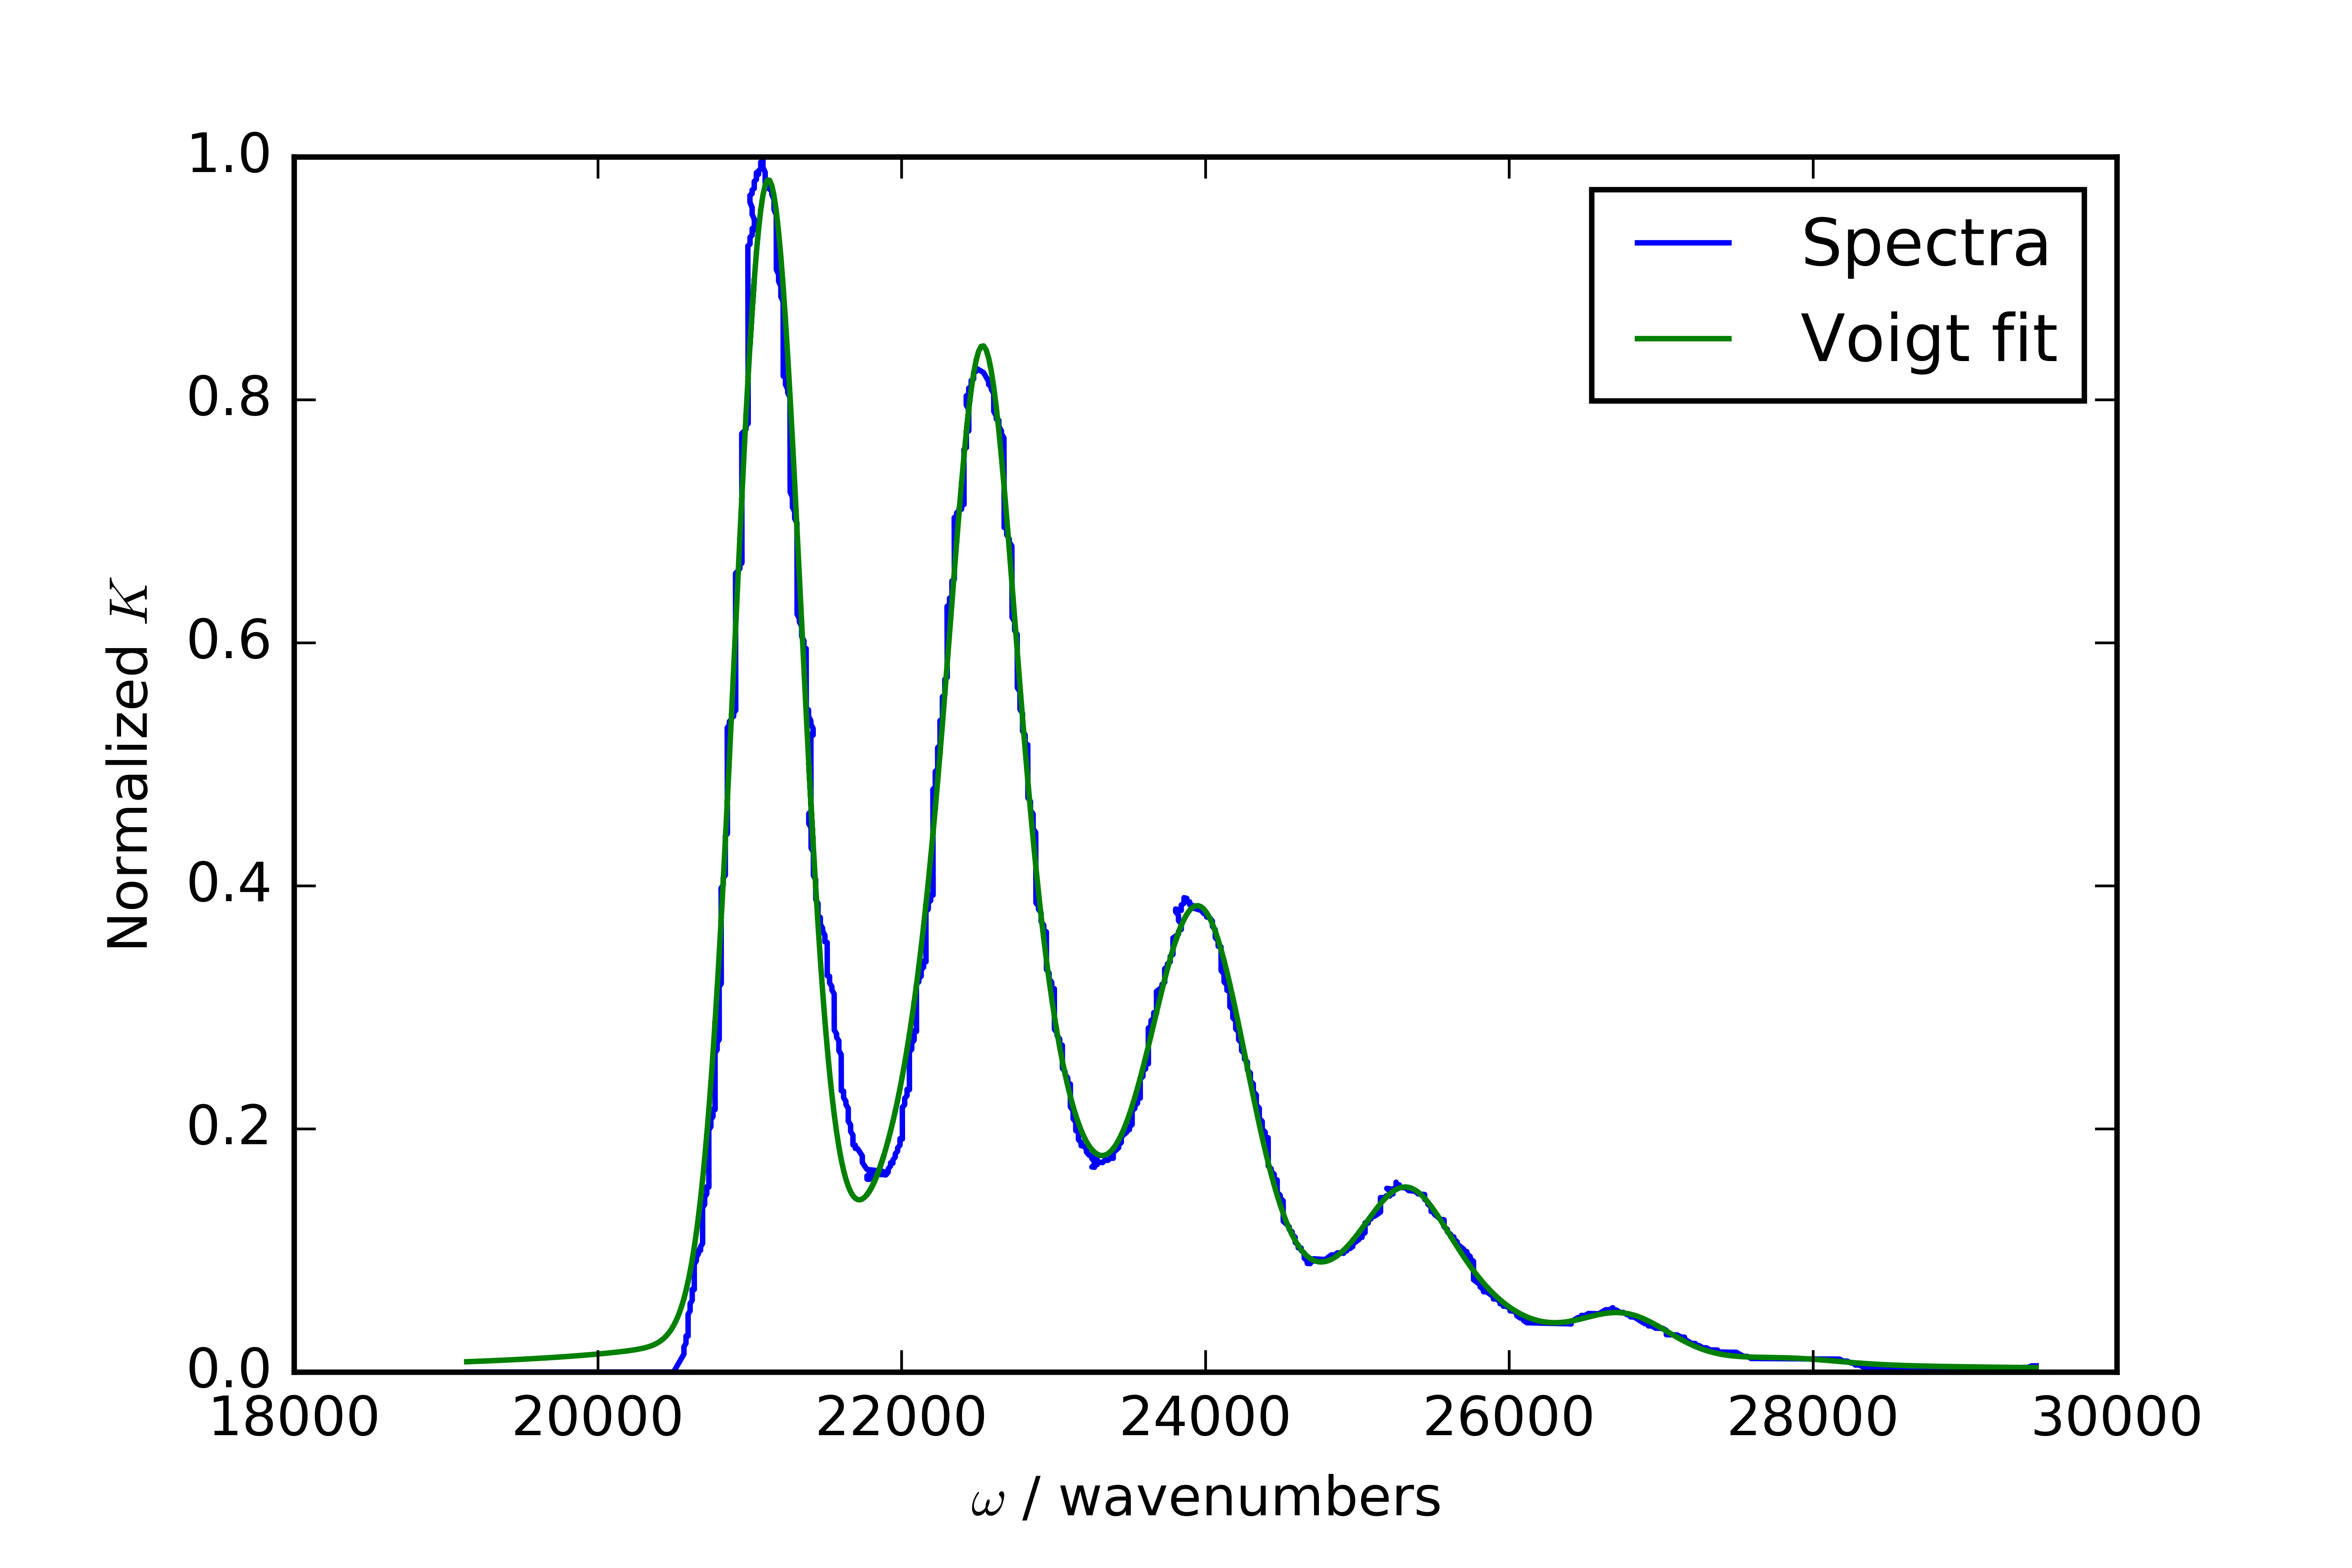
\includegraphics[width=1.0\columnwidth]{dcm_spectra_fit.png}
   \caption{The fit for Voigt line-shapes to the spectra of tetracene in dichloromethane from Ref. ~\cite{TetraceneDichloromethane}}
	\label{fig:dcm_fit}
\end{figure}

\begin{figure}
   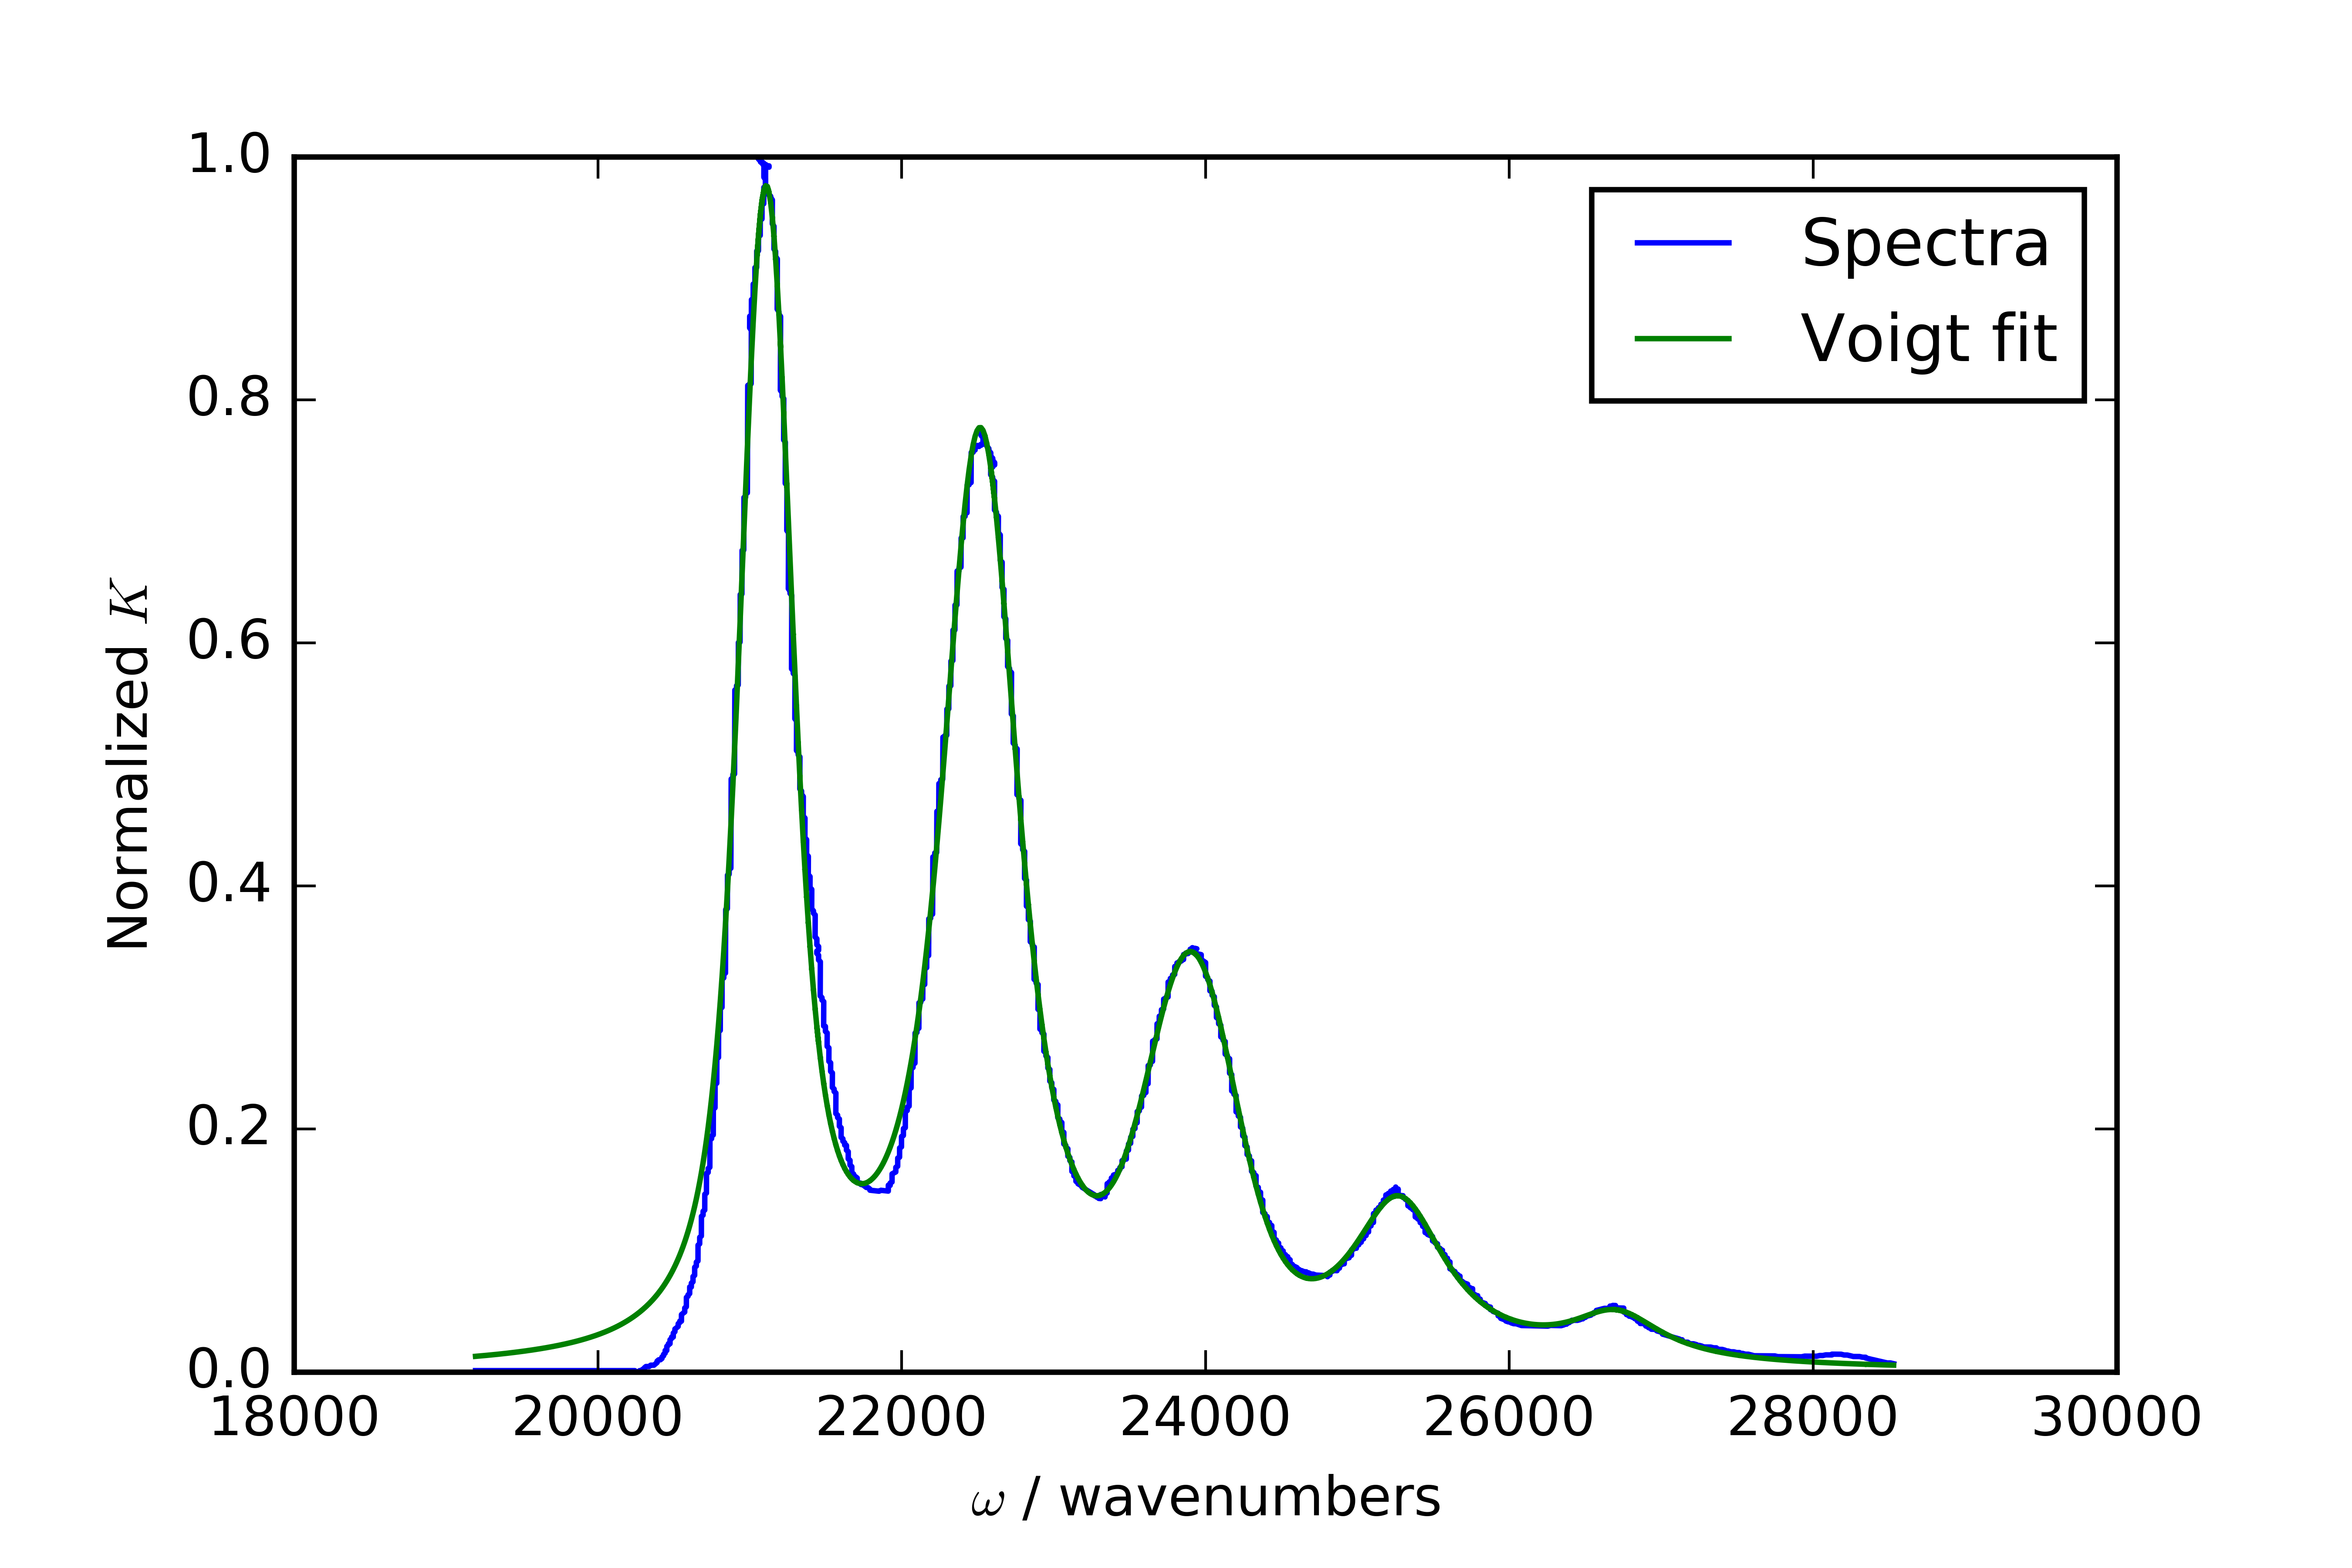
\includegraphics[width=1.0\columnwidth]{toluene_spectra_fit.png}
   \caption{The fit for Voigt line-shapes to the spectra of tetracene in toluene from Ref.~\cite{TetraceneToluene}}
	\label{fig:toluene_fit}
\end{figure}

\begin{table}
 \begin{tabular}{lcc}
 \hline
 Parameter & DCM & Toluene \\
 \hline
 $V_0$ / cm$^{-1}$  & 20421.87 &  20420.06\\
 $\omega_e$ / cm$^{-1}$ & 1404.74 & 1388.87 \\
 $\chi_e \omega_e$ / cm$^{-1}$ & -.9501 &  -1.5 \\
 $r^2$ & 0.9999 &  1.0000 \\
 \hline
\end{tabular}
\caption{ Fit of the calculated peak heights to a Morse potential model.  Because of the small value of $\chi_e \omega_e$ relative to $\omega_e$, we conclude that the harmonic approximation is reasonable for this system.}
% [Al\'an, I couldn't find the specific package you were talking about but I think I got the right formatting based off of a PRL I found.  Let me know!]
\label{table:energyFit}
\end{table}


\begin{table}
 \begin{tabular}{lcc}
 \hline
 \textbf{Parameter} & \textbf{DCM} & \textbf{Toluene} \\
 \hline
 $S_{\text{Condon}}$ & 1.52 & 1.185 \\
 $r^2_{\text{Condon}}$ & .743 & .829\\
 \hline
 $S_{ (2) }$ & 1.263  &  1.201 \\
 $c'_{ 2 }$ & -0.067  &  0.006 \\
 $\theta'_{ 2 } / \pi $& 6.283  &  0.000 \\
 $r^2_{ (2) }$ & 0.833  &  0.830 \\
 \hline
 $S_{ (1, 3) }$ & 1.174  &  1.185 \\
 $c'_{ 1 }$ & -0.277  &  0.222 \\
 $\theta'_{ 1 } / \pi $& 4.206  &  5.388 \\
 $c'_{ 3 }$ & -0.237  &  0.180 \\
 $\theta'_{ 3 } / \pi $& 1.251  &  1.712 \\
 $r^2_{ (1, 3) }$ & 0.977  &  1.000 \\
 \hline
\end{tabular}
\caption{Fit of certain parameters}
\label{table:peakFit}
\end{table}

Then to fit to Equation \ref{eqn:HDef}, we employed a trust region reflective algorithm least-squares fitting procedure as implemented in the Scipy package by fitting to the ~\cite{scipy,numpy}.  Because there are multiple solutions for $c$ and $\theta$ for all orders, we include a small regularization term in the fitting procedure to keep the solutions close to the Condon value of $S$.

Our method was unable to find a better fit than the Condon solution for for the (1) model, but (2) gave interesting results as did (1,3).  We expect odd-polynomials to be the most physically relevant because of the broken symmetry when the molecule gets excited; we expect the molecule to preferentially absorb to the excited state when the nuclear configuration is closer to the shape of the excited state. $H_{(2)}(k,0)$ and $H_{(1,3)}(k,0)$ and give the results of their fitting in Table \ref{table:peakFit} and an example of one of these fits is in Figure \ref{fig:dcm_ratio13_fit} and \ref{fig:toluene_ratio13_fit}.

\begin{figure}
   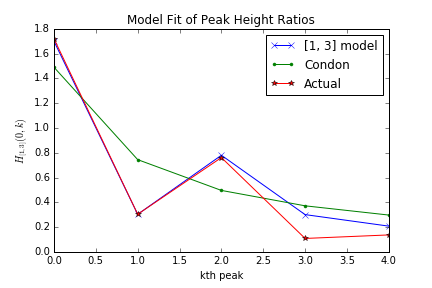
\includegraphics[width=1.0\columnwidth]{dcm_ratio_fit_13.png}
   \caption{The Voigt-derived values of $H(0,k)$ from tetracene in DCM, fit to the model for $H_{(1,3)}(0,k)$ and a purely Condon model.  Note that the Condon model does not fit the trend very well at all whereas the non-Condon model tracks the trend very well.}
	\label{fig:dcm_ratio13_fit}
\end{figure}
\begin{figure}
   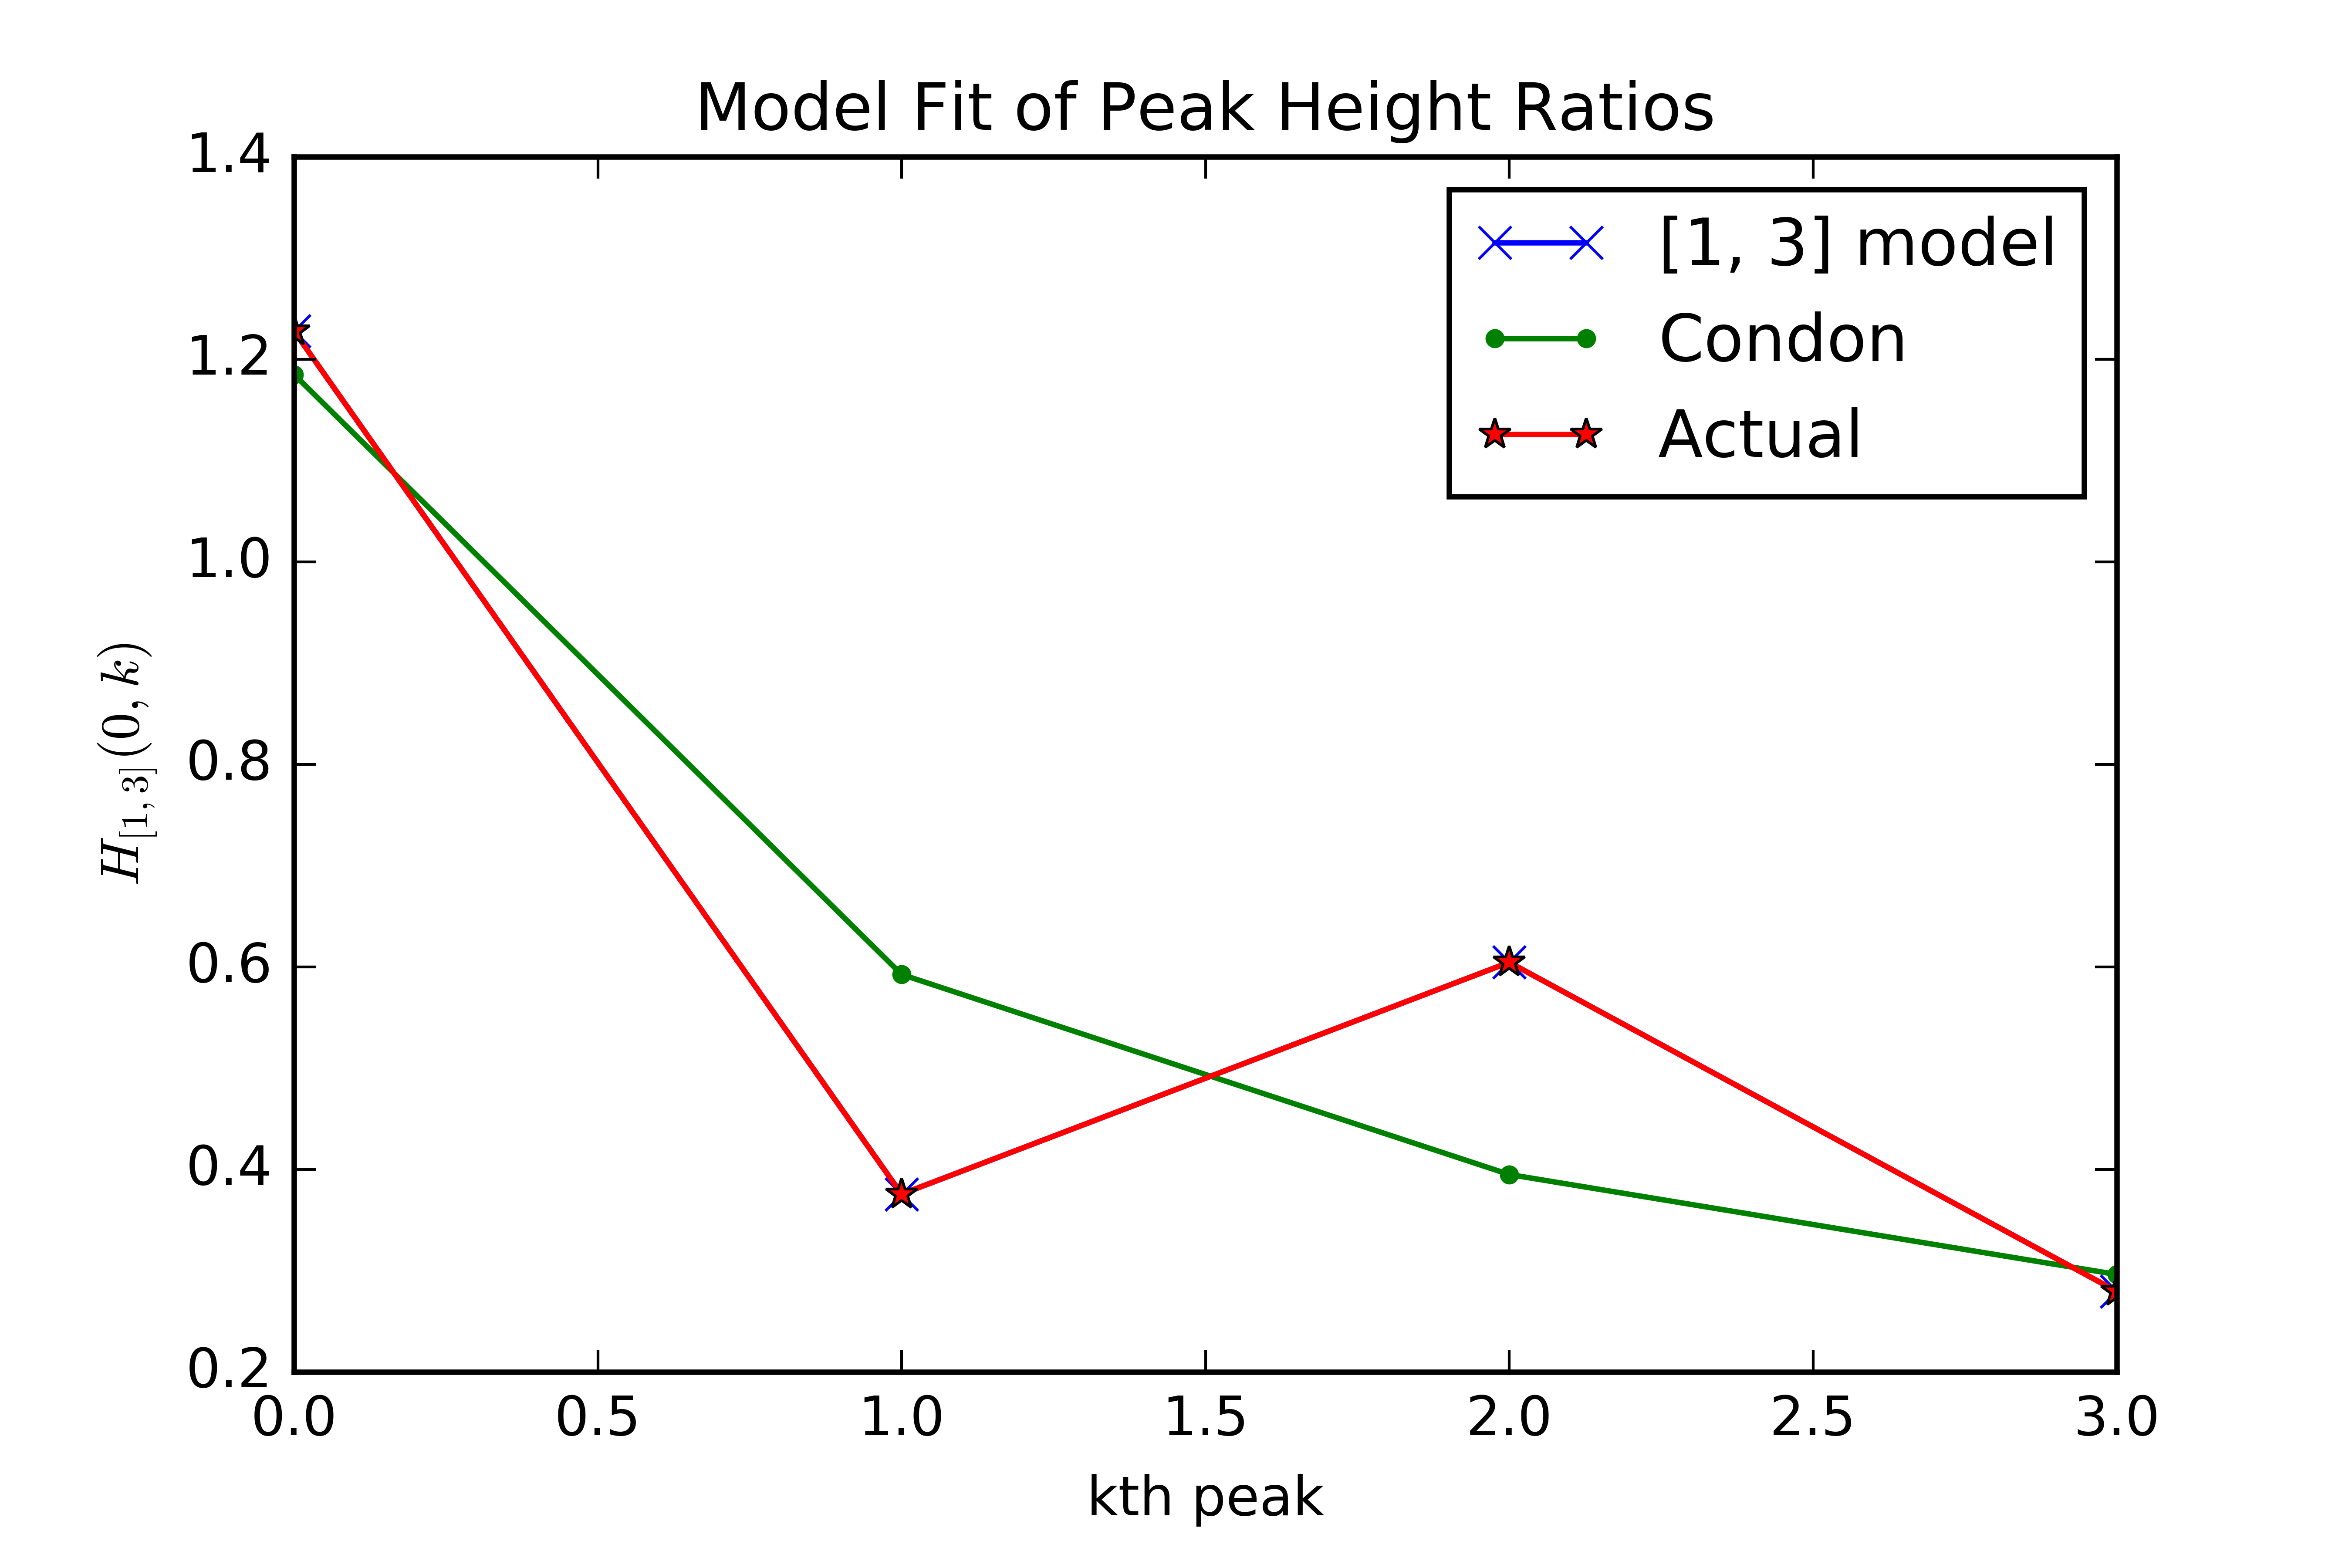
\includegraphics[width=1.0\columnwidth]{toluene_ratio_fit_13.png}
   \caption{The Voigt-derived values of $H(0,k)$ from tetracene in toluene, fit to the model for $H_{(1,3)}(0,k)$ and a purely Condon model.  Note that the Condon model does not fit the trend very well at all whereas the non-Condon model tracks the trend very well.}
	\label{fig:toluene_ratio13_fit}
\end{figure}

We can also look at the functional form of $\mu(x)$ from transforming $c'$ into $c$.  The result of this for (1,3) is shown in Figure \ref{fig:mu_fit_comparison}.  Despite the slightly different values for $c'$ and $S$ for the (1,3) correction, the derived transition dipole moments seem roughly similar.

\begin{figure}
   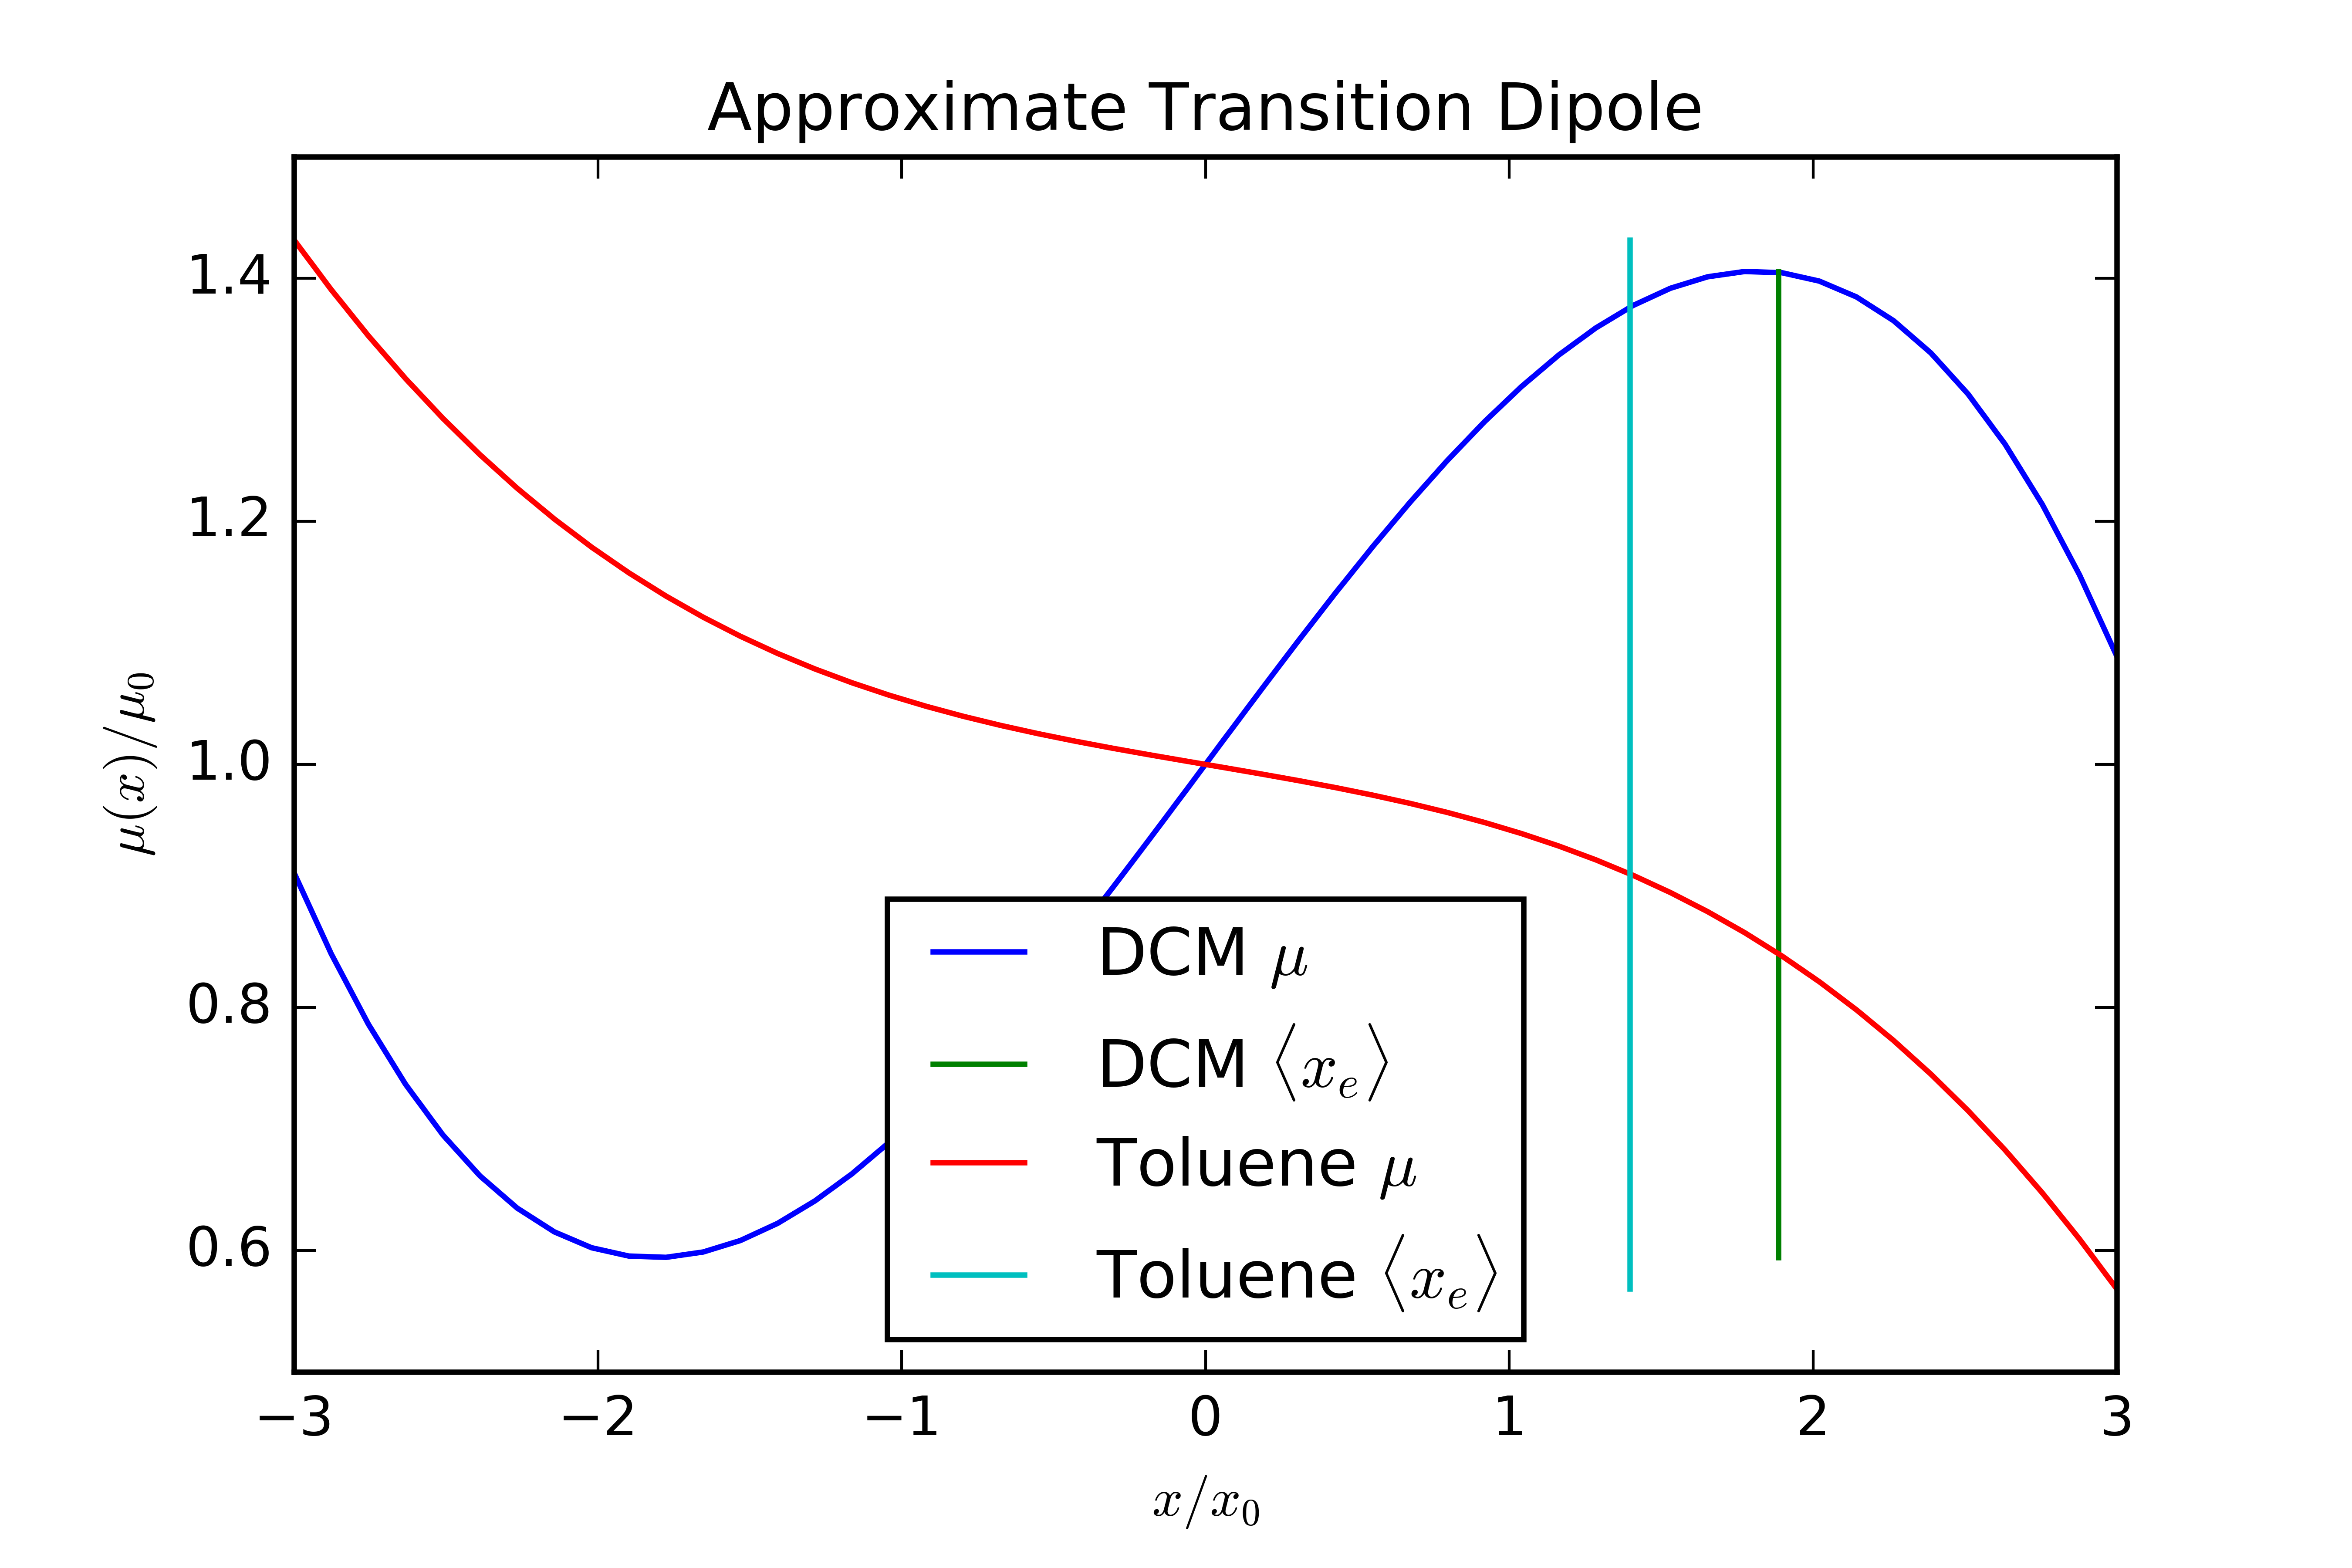
\includegraphics[width=1.0\columnwidth]{dipole_comparison_13.png}
   \caption{The fitted functional form for the transition dipole moment calculated for the Voigt-derived values of $H(0,k)$ to the model for $H_{(1,3)}(0,k)$.}
	\label{fig:mu_fit_comparison}
\end{figure}


\section{Conclusion}
We have developed a method to provide estimates of the vibrational structure of an electronic transition dipole moment by fitting to the linear electronic absorption spectrum and applied this method to tetracene in two different solvents.  We note that linear expansions for the transition dipole variation can be extracted from simple spectra in solution. Further work on e.g. molecular spectroscopic databases will be useful to further explore the magnitude of the corrections studied in this work.


\section{Acknowledgments}
We acknowledge the support from the Center for Excitonics, an Energy Frontier Research Center funded by the U.S. Department of Energy under award DE-SC0001088 (Solar energy conversion process).  The authors also wish to thank Jacob Krich for discussions and Alex Eisfeld for his commentary on this manuscript.
